\documentclass[conference]{IEEEtran}
\IEEEoverridecommandlockouts
% The preceding line is only needed to identify funding in the first footnote. If that is unneeded, please comment it out.
\usepackage{cite}
\usepackage{amsmath,amssymb,amsfonts}
\usepackage{algorithmic}
\usepackage{graphicx}
\usepackage{textcomp}
\usepackage{xcolor}

\def\BibTeX{{\rm B\kern-.05em{\sc i\kern-.025em b}\kern-.08em
    T\kern-.1667em\lower.7ex\hbox{E}\kern-.125emX}}
\begin{document}

\title{
    CMOS INVERTERS AND THEIR VOLTAGE TRANSFER CHARACTERISTICS (VTC) DESIGN, 
    SIMULATION, EXPERIMENTAL TEST, AND ANALYSIS\\
}

\author{
    \IEEEauthorblockN{1\textsuperscript{st} Anthony Jerez}
    \IEEEauthorblockA{\textit{College of Electrical and Computer Engineering} \\
    \textit{California State University, Northridge}\\
    Northridge, CA \\
    anthony.jerez.156@my.csun.edu}
    \and
    \IEEEauthorblockN{2\textsuperscript{nd} Syar Humayun}
    \IEEEauthorblockA{\textit{College of Electrical and Computer Engineering} \\
    \textit{California State University, Northridge}\\
    Northridge, CA}
}

\maketitle

\begin{abstract}
    Upon studying the basic structure and function of the NMOS and PMOS transistor,
    we study its voltage transfer characteristics when implemented as a complimentary 
    MOS (CMOS). Noise margins, propagation delay and the switching threshold ($V_m$)
    are all looked at in this report. Simulations done in Pspice are shown 
    as well as their experiemental counterparts.
\end{abstract}

\begin{IEEEkeywords}
    CMOS, NMOS, PMOS, High \& Low Noise Margins ($NM_H$ and $NM_L$ respectively), 
    Propagation Delay, Switching Threshold ($V_m$).
\end{IEEEkeywords}

\section{Introduction}
    The complimentary MOS or CMOS is one of the most fundamental implementations 
    of the CMOS and PMOS transistors. CMOS digital circuits utitlize NMOS and 
    PMOS transistors operating as switches. 
    
    \begin{center}
        \centerline{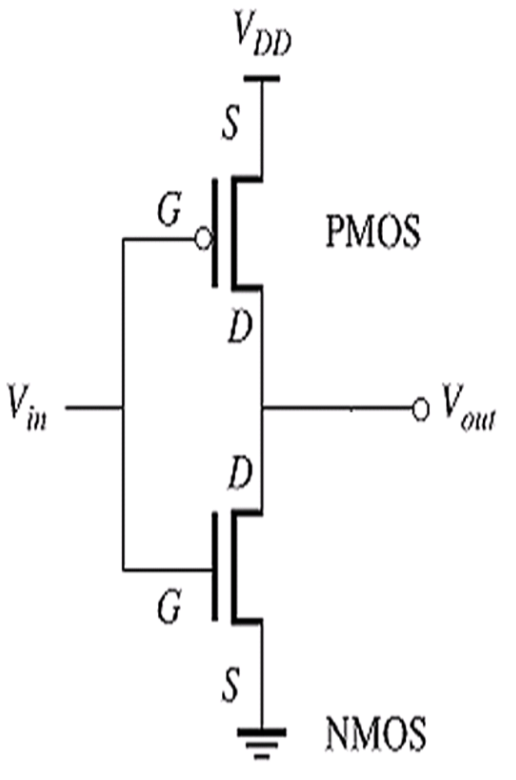
\includegraphics[scale = 0.4]{figures/CMOS_schematic.png}}
        Figure 1. CMOS inverter schematic
    \end{center}

    An NMOS transistor will behave similar to a closed switch, exhibiting a small 
    resistance between the drain and source when its gate voltage is "high" (logic 1). 
    Conversely, when the gate voltage is "low" (logic 0), the transistor acts as open 
    switch and the transistor is cut-off. The PMOS works in a similar fashion only in 
    reverse. When we use these inverters in this way, with the PMOS on top of the NMOS 
    (shown in figure 3), the CMOS will invert the input which is what is demonstrated in 
    figure 4.

    \begin{center}
        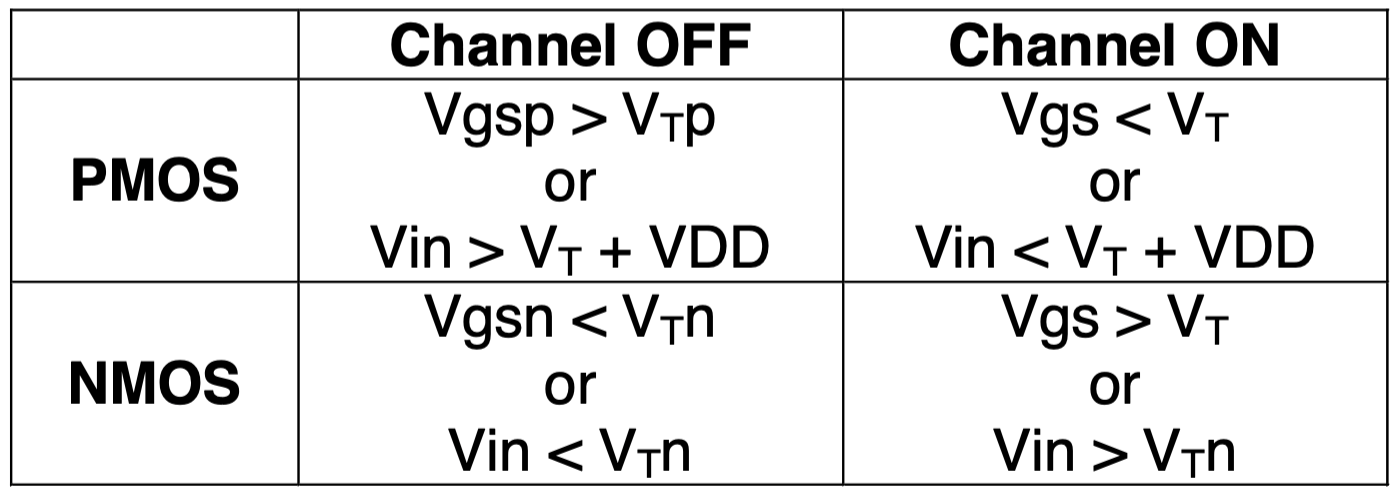
\includegraphics[scale = 0.32]{figures/tabel1.png}
        Figure 2. Relationship between the gate-source voltage $V_{gs}$ and the 
        threshold voltage $V_t$
    \end{center}

    \subsection{Propagation Delay and Noise Margins}
    The propagation delay describes the amount of time between the change of the input 
    and output at the 50\% point. These measurments are taken when the output changes 
    from high to low and from low to high since the propagation delays are usually not 
    equal. The two values are then averaged out, giving us the following equation:
    \begin{align}
        \tau_P = \frac{\tau_{PHL} + \tau_{PLH}}{2} 
    \end{align}
    Noise margins describe a "safety margin" to prevent the circuit from producing 
    incorrect outputs due to a noisy input signal. Noise margins tell us the ranges 
    we should be in to allow the circuit to work properly given a certain amount of 
    noise. Noise margins are given for both high and low input levels are are given 
    by:
    \begin{align}
        NM_L = V_{IL} - V_{OL}\\
        NM_H = V_{OH} - V_{IH}
    \end{align}

\section{ PROCEDURES, SIMULATION AND EXPERIMENTAL SET-UP}

\subsection{Case 1 (100kHz $\leq$ f $\leq$ 200kHz)}

\begin{center}
    \centerline{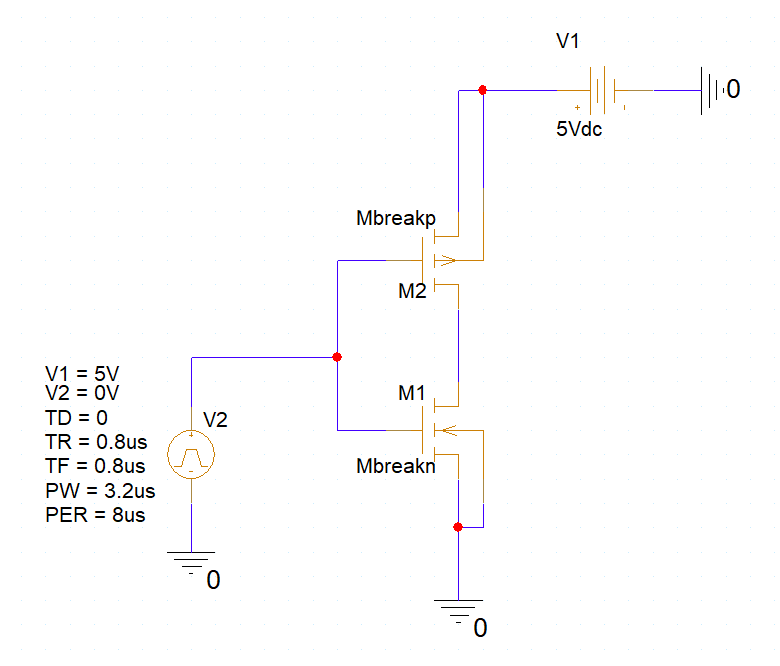
\includegraphics[scale = 0.43]{figures/case1_circuit.png}}
    Figure 3. Case I - 5V, 122kHz Rectangular input
\end{center}

\begin{center}
    \centerline{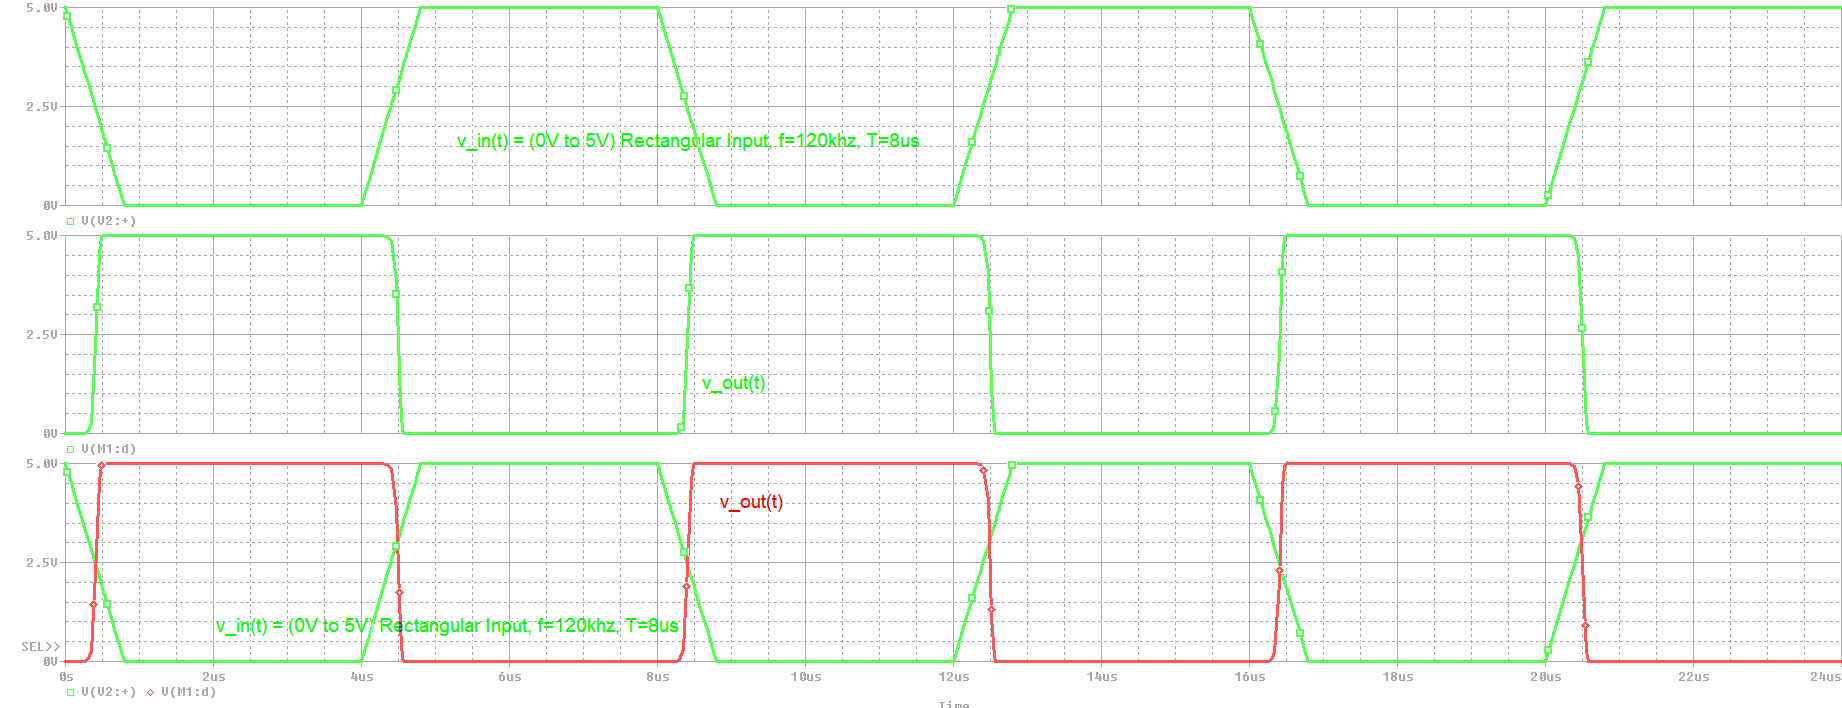
\includegraphics[scale = 0.18]{figures/case1_results1.png}}
    Figure 4. Case I - 5V, 124kHz Rectangular input, simulation
\end{center}

\begin{center}
    \centerline{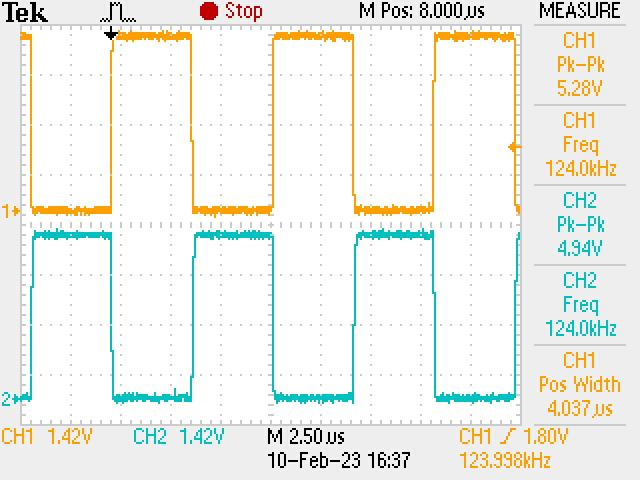
\includegraphics[scale = 0.9]{figures/case1_lab_result.JPG}}
    Figure 5. Case I - 5V, 124kHz Rectangular input, experpimental
\end{center}

\begin{center}
    \centerline{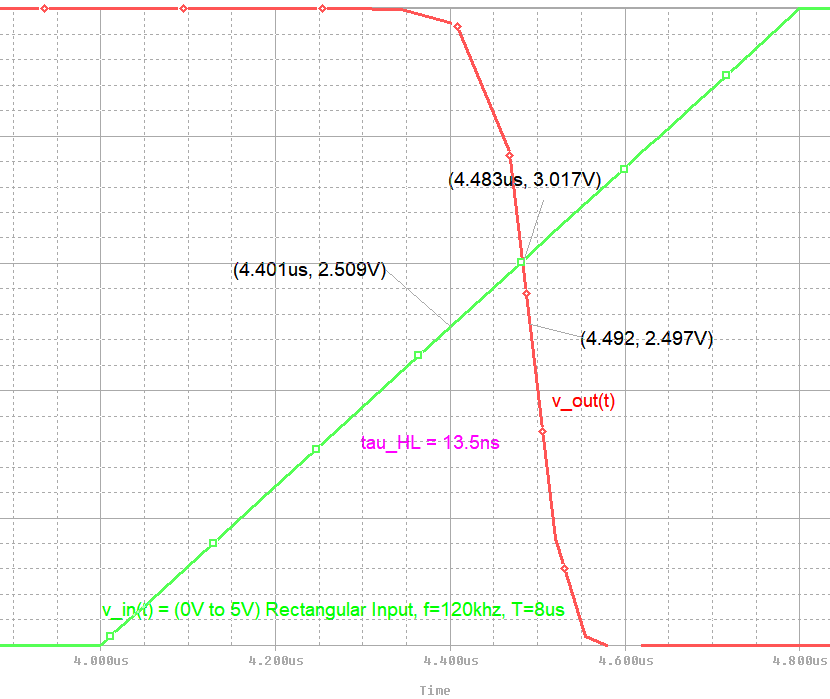
\includegraphics[scale = 0.39]{figures/case1_results_HL.png}}
    Figure 6. Case I - 5V, 122kHz, VTC simulation (High to Low)
\end{center}

\begin{center}
    \centerline{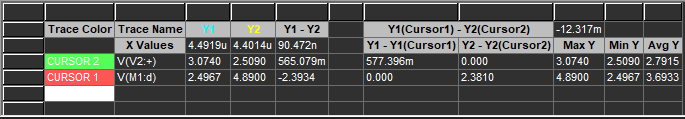
\includegraphics[scale = 0.45]{figures/case1_results_HL_data.png}}
    Figure 7. Case I - 5V, 122kHz, VTC simulation data (High to Low)
\end{center} 

Figure 7 shows propagation delay at the 50\% point when the output goes from 
high to low. There is a typo in Fig. 6 for the value of tau, but we can see that
from the data, there is about 90ns between the input and output which will be our 
$\tau_{PHL}$ value.

\begin{center}
    \centerline{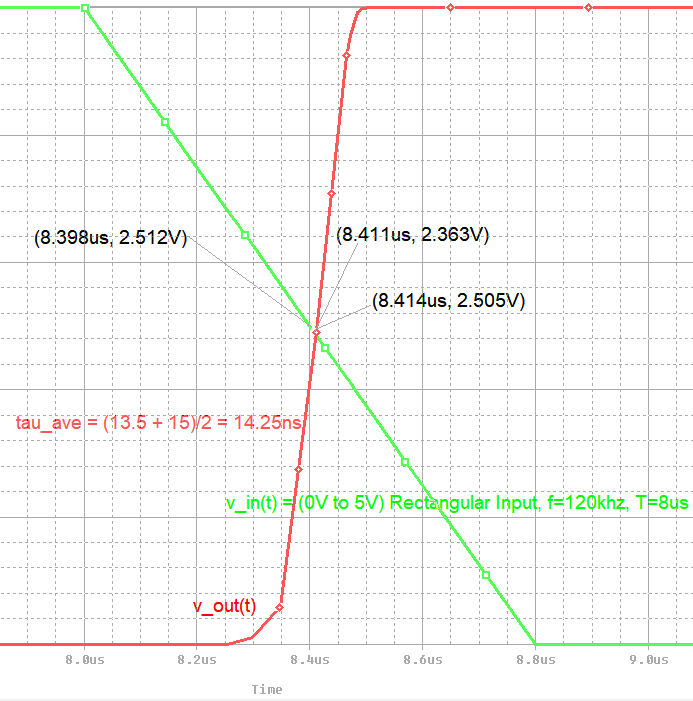
\includegraphics[scale = 0.45]{figures/case1_results_LH.png}}
    Figure 8. Case I - 5V, 122kHz, VTC simulation (Low to High)
\end{center} 

\begin{center}
    \centerline{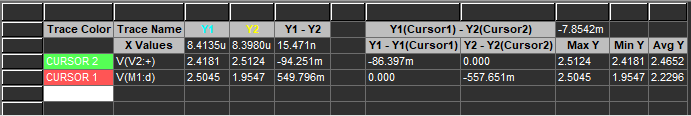
\includegraphics[scale = 0.45]{figures/case1_results_LH_data.png}}
    Figure 9. Case I - 5V, 122kHz, VTC simulation data (Low to High)
\end{center} 

Here we see that $\tau_{PLH} = 15$ns, giving us a propagation delay of 
$\tau_P = (90ns + 15ns)/2 = 52.5ns$

\begin{center}
    \centerline{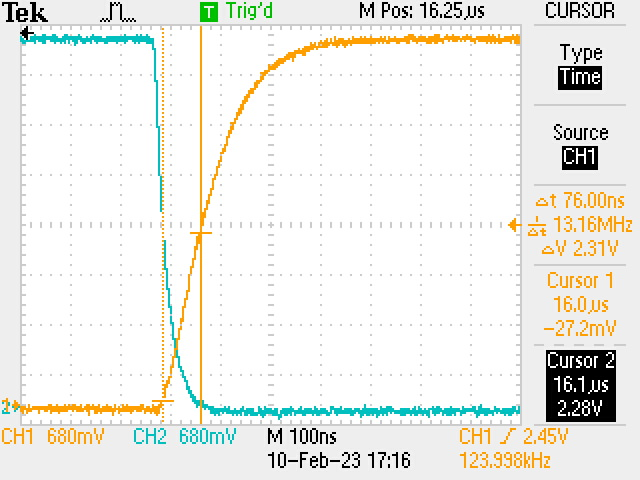
\includegraphics[scale = 0.9]{figures/case1_HL_experimental.JPG}}
    Figure 10. Case I - 5V, 124kHz, VTC experimental (High to Low)
\end{center} 

\begin{center}
    \centerline{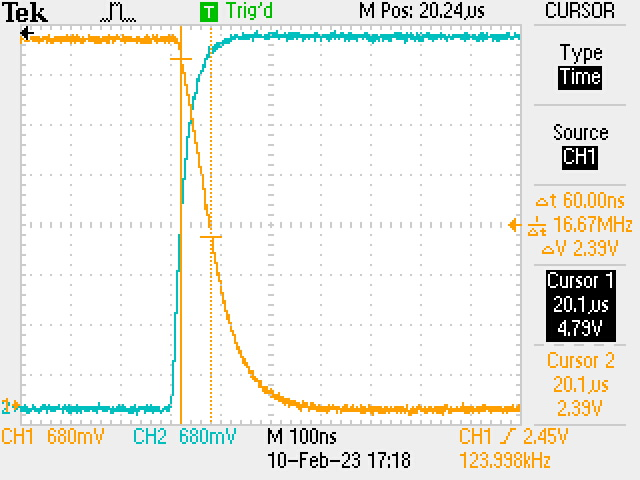
\includegraphics[scale = 0.9]{figures/case1_LH_experimental.JPG}}
    Figure 11. Case I - 5V, 124kHz, VTC experiemtnal (Low to High)
\end{center} 

For the experimental case, we see that $\tau_{PHL} = 76ns$ and 
$\tau_{PLH} = 60ns$, giving us a propagation delay of $\tau_P = 68ns$

\subsection{Case 2 (300kHz $\leq$ f $\leq$ 500kHz)}

\begin{center}
    \centerline{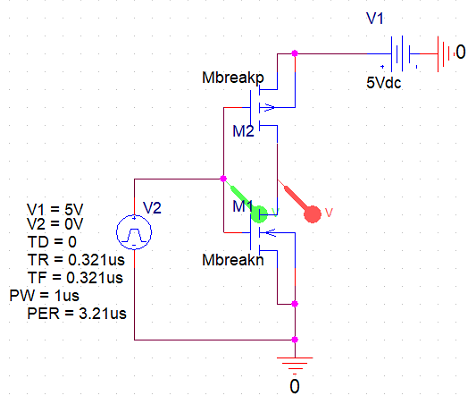
\includegraphics[scale = 0.7]{figures/case2_circuit.png}}
    Figure 12. Case II - 5V Square input, f = 312kHz and t = 3.21us
\end{center}

\begin{center}
    \centerline{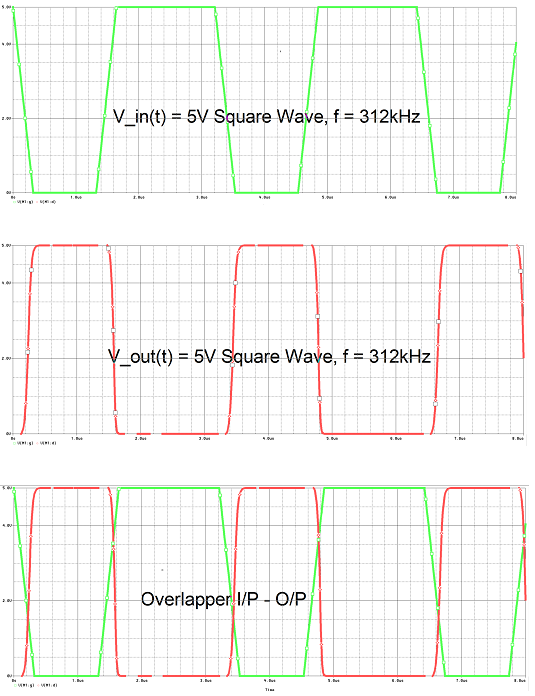
\includegraphics[scale = 0.5]{figures/case2_results1.png}}
    Figure 13. Case II - 5V Square input, f = 312kHz and t = 3.21us, simulation
\end{center}

\begin{center}
    \centerline{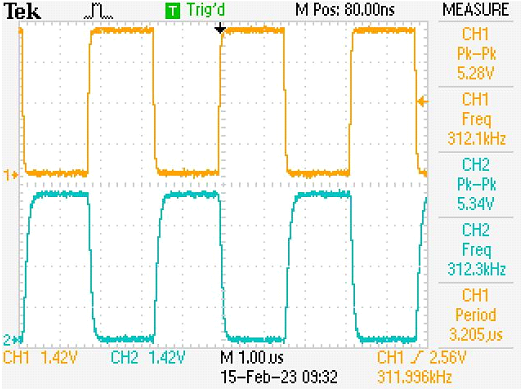
\includegraphics[scale = 0.6]{figures/case2_lab_results.png}}
    Figure 14. Case II - 5V Square input, f = 312kHz and t = 3.21us, experimental
\end{center}

\begin{center}
    \centerline{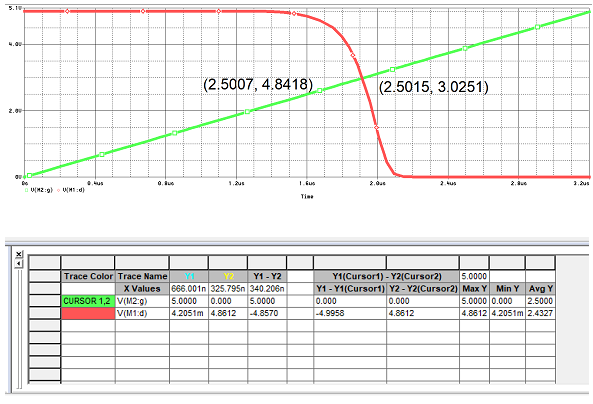
\includegraphics[scale = 0.55]{figures/case2_results_HL.png}}
    Figure 15. Case II - 5V, f = 312kHz, VTC simulation (High to Low)
\end{center}

\begin{center}
    \centerline{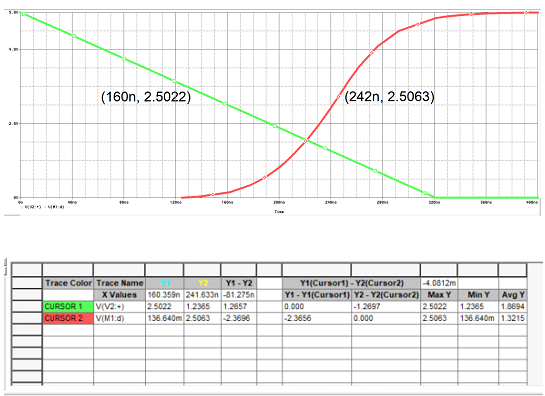
\includegraphics[scale = 0.6]{figures/case2_results_LH.png}}
    Figure 16. Case II - 5V, f = 312kHz, VTC simulation (Low to High)
\end{center}

\begin{center}
    \centerline{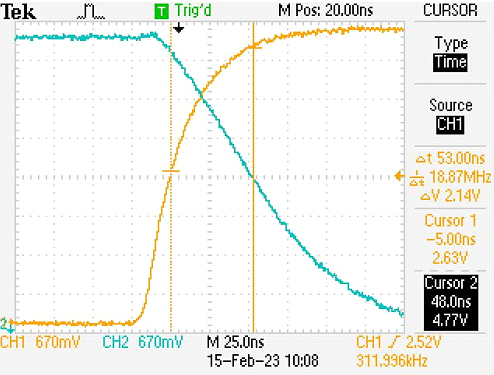
\includegraphics[scale = 0.6]{figures/case2_HL_experimental.png}}
    Figure 17. Case II - 5V, f = 312kHz, VTC Experimental (High to Low)
\end{center}

\begin{center}
    \centerline{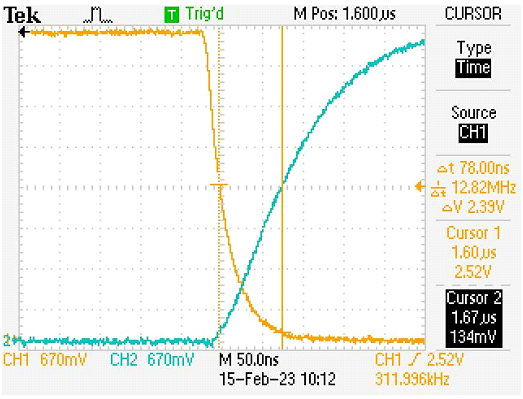
\includegraphics[scale = 0.6]{figures/case2_LH_experimental.png}}
    Figure 18. Case II - 5V, f = 312kHz, VTC Experimental (Low to High)
\end{center}

\subsection{Case 3 (600kHz $\leq$ f $\leq$ 800kHz)}

\begin{center}
    \centerline{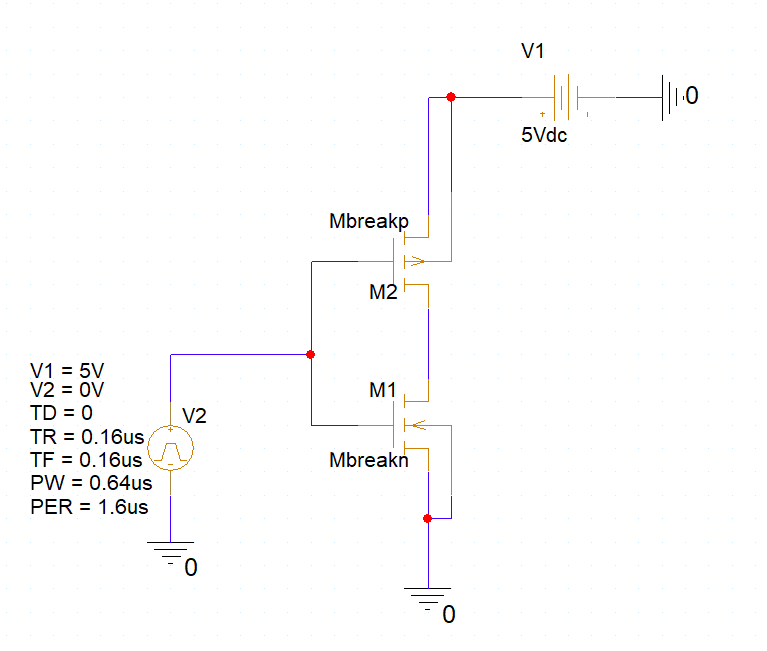
\includegraphics[scale = 0.43]{figures/case3_circuit.png}}
    Figure 19. Case III - 5V, 622kHz Rectangular input
\end{center}

\begin{center}
    \centerline{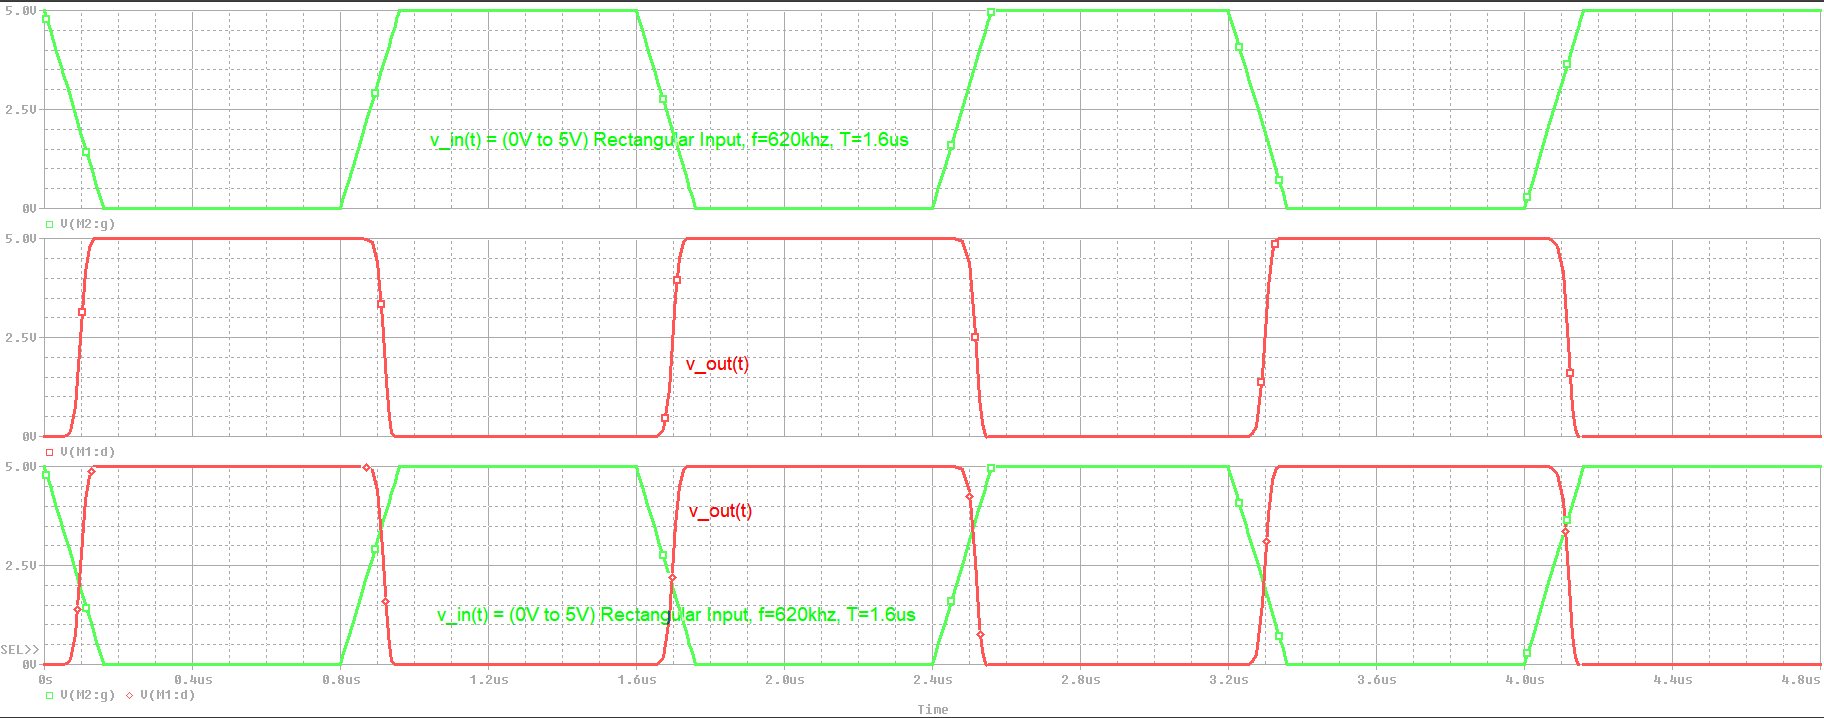
\includegraphics[scale = 0.18]{figures/case3_results1.png}}
    Figure 20. Case III - 5V, 622kHz Rectangular input, simulation
\end{center}

\begin{center}
    \centerline{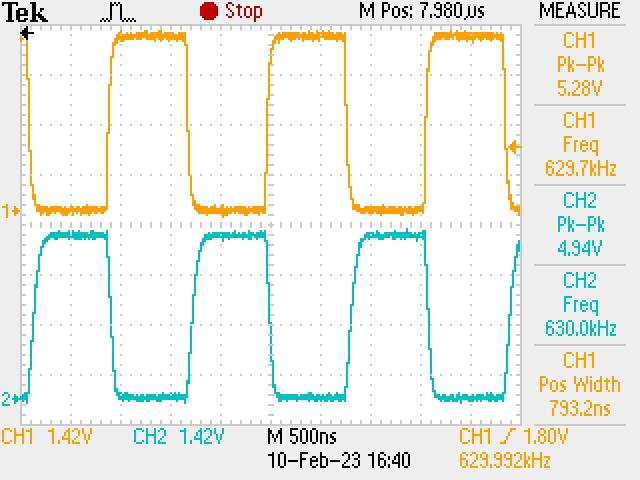
\includegraphics[scale = 0.9]{figures/case3_lab_result.JPG}}
    Figure 21. Case III - 5V, 630kHz Rectangular input, experpimental
\end{center}

\begin{center}
    \centerline{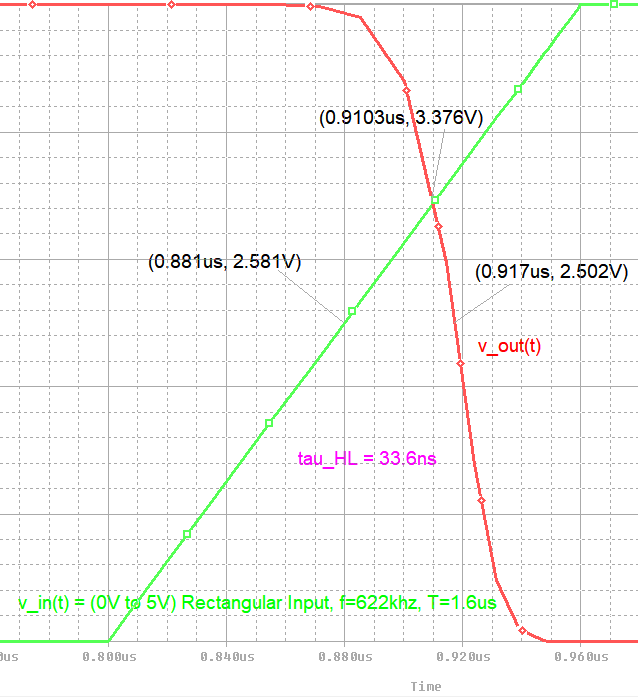
\includegraphics[scale = 0.47]{figures/case3_results_HL.png}}
    Figure 22. Case III - 5V, 622kHz, VTC simulation (High to Low)
\end{center}

\begin{center}
    \centerline{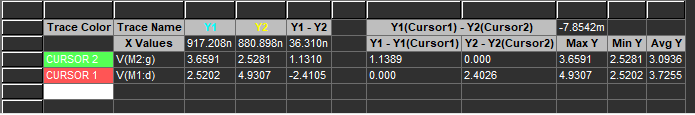
\includegraphics[scale = 0.5]{figures/case3_results_HL_data.png}}
    Figure 23. Case III - 5V, 622kHz, VTC simulation data (High to Low)
\end{center} 

\begin{center}
    \centerline{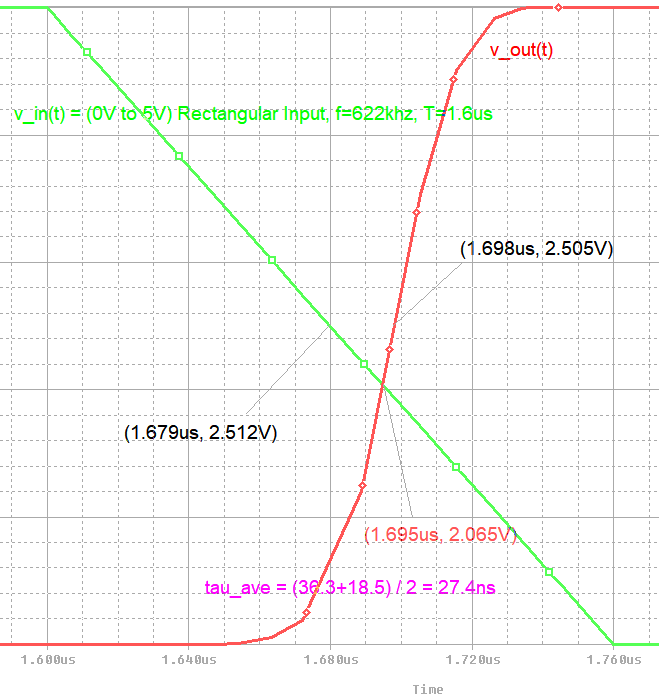
\includegraphics[scale = 0.48]{figures/case3_results_LH.png}}
    Figure 24. Case III - 5V, 622kHz, VTC simulation (Low to High)
\end{center} 

\begin{center}
    \centerline{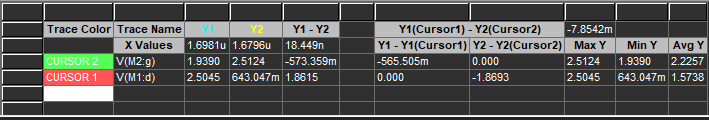
\includegraphics[scale = 0.5]{figures/case3_results_LH_data.png}}
    Figure 25. Case III - 5V, 622kHz, VTC simulation data (Low to High)
\end{center}

Here we see that $\tau_{PLH} = 18$ns, giving us a propagation delay of 
$\tau_P = (36ns + 18ns)/2 = 27ns$

\begin{center}
    \centerline{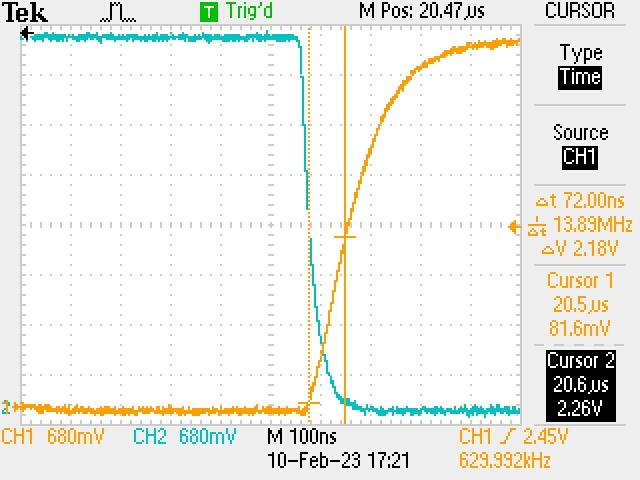
\includegraphics[scale = 0.9]{figures/case3_HL_experimental.JPG}}
    Figure 26. Case III - 5V, 624kHz, VTC experimental (High to Low)
\end{center} 

\begin{center}
    \centerline{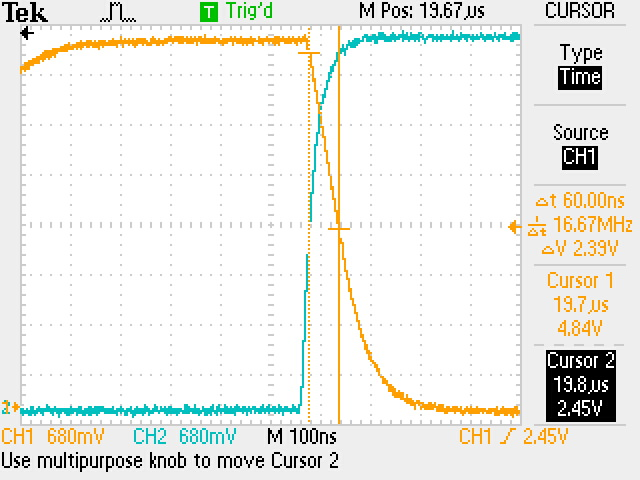
\includegraphics[scale = 0.9]{figures/case3_LH_experimental.JPG}}
    Figure 27. Case III - 5V, 624kHz, VTC experiemtnal (Low to High)
\end{center} 

For the experimental case, we see that $\tau_{PHL} = 72ns$ and 
$\tau_{PLH} = 60ns$, giving us a propagation delay of $\tau_P = 66ns$

\subsection{Case 4 (900kHz $\leq$ f $\leq$ 1.2MHz)}

\begin{center}
    \centerline{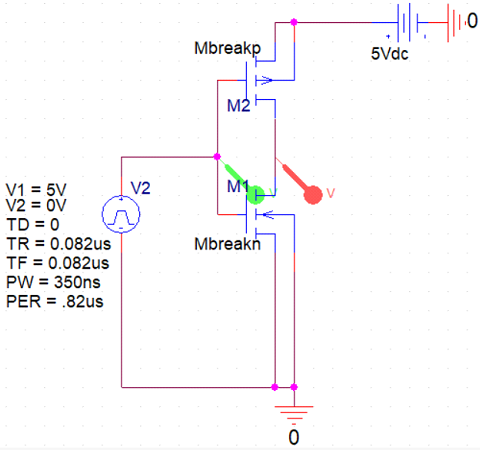
\includegraphics[scale = 0.6]{figures/case4_circuit.png}}
    Figure 28. Case IV - 5V Square input, f = 1.22MHz and t = 0.82us
\end{center}

\begin{center}
    \centerline{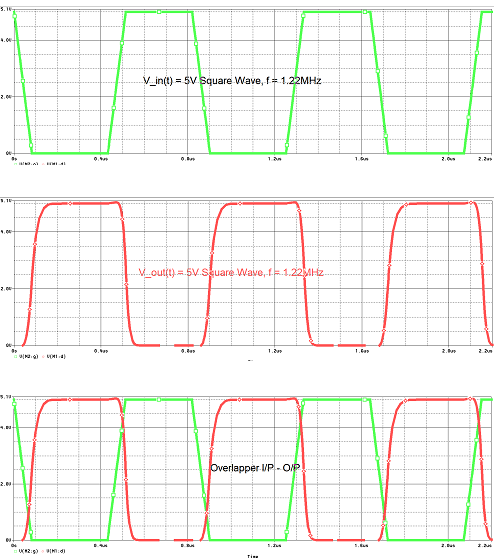
\includegraphics[scale = 0.6]{figures/case4_results1.png}}
    Figure 29. Case IV - 5V Square input, f = 1.22MHz and t = 0.82us, simulation
\end{center}

\begin{center}
    \centerline{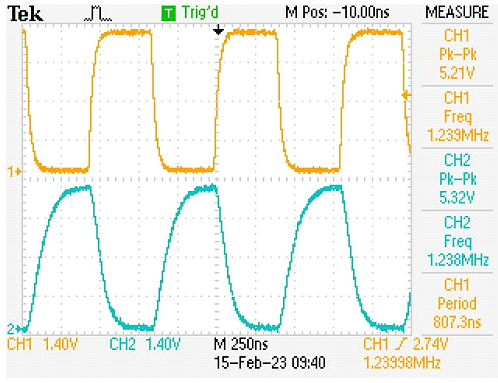
\includegraphics[scale = 0.6]{figures/case4_lab_results.png}}
    Figure 30. Case IV - 5V Square input, f = 1.22MHz and t = 0.82us, experimental
\end{center}

\begin{center}
    \centerline{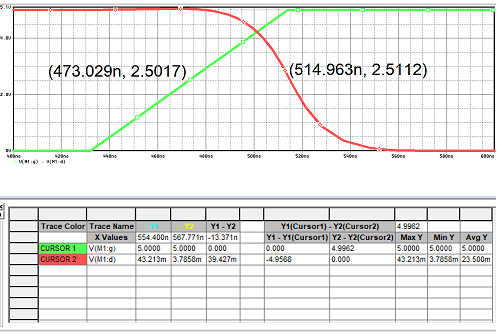
\includegraphics[scale = 0.6]{figures/case4_results_HL.png}}
    Figure 31. Case IV - 5V, f = 1.22MHz, VTC simulation (High to Low)
\end{center}

\begin{center}
    \centerline{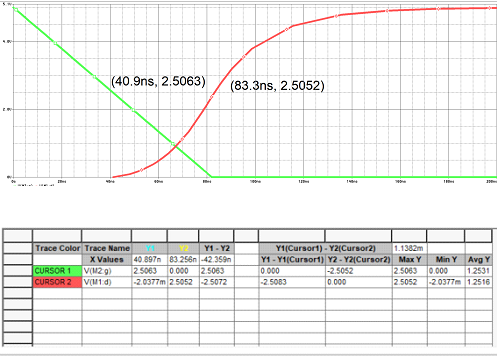
\includegraphics[scale = 0.65]{figures/case4_results_LH.png}}
    Figure 32. Case IV - 5V, f = 1.22MHz, VTC simulation (Low to High)
\end{center}

\begin{center}
    \centerline{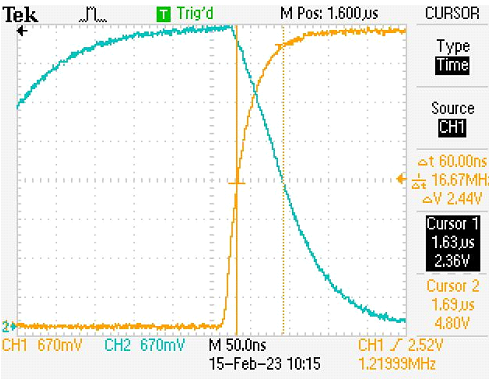
\includegraphics[scale = 0.6]{figures/case4_HL_experimental.png}}
    Figure 33. Case IV - 5V, f = 1.22MHz, VTC Experimental (High to Low)
\end{center}

\begin{center}
    \centerline{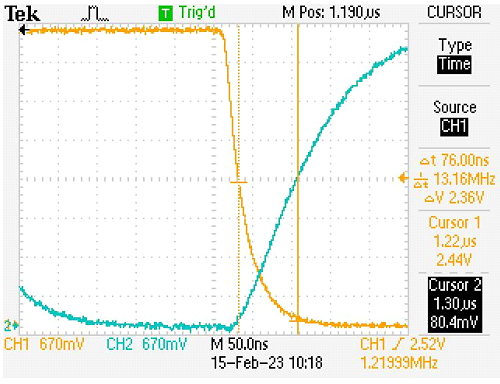
\includegraphics[scale = 0.6]{figures/case4_LH_experimental.png}}
    Figure 34. Case IV - 5V, f = 1.22MHz, VTC Experimental (Low to High)
\end{center}

\subsection{Ramp Case 1 (80kHz $\leq$ f $\leq$ 100kHz)}

\begin{center}
    \centerline{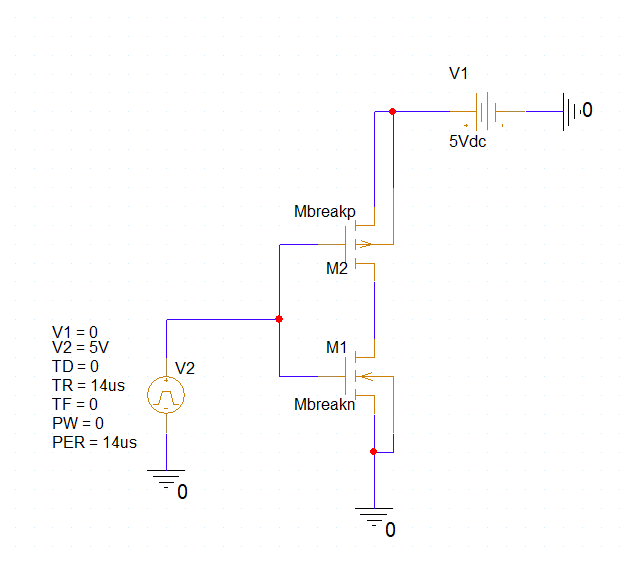
\includegraphics[scale = 0.51]{figures/rampcase1_circuit.png}}
    Figure 35. Ramp Case I - 5V, 80kHz Ramp input
\end{center}

\begin{center}
    \centerline{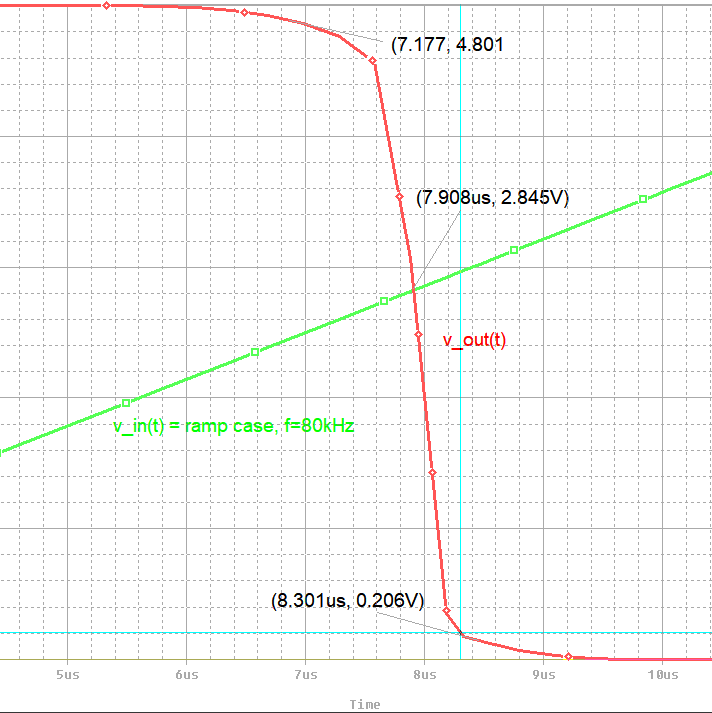
\includegraphics[scale = 0.42]{figures/rampcase1_results.png}}
    Figure 36. Ramp Case I - 5V, 80kHz Ramp input, simulation
\end{center}

\begin{center}
    \centerline{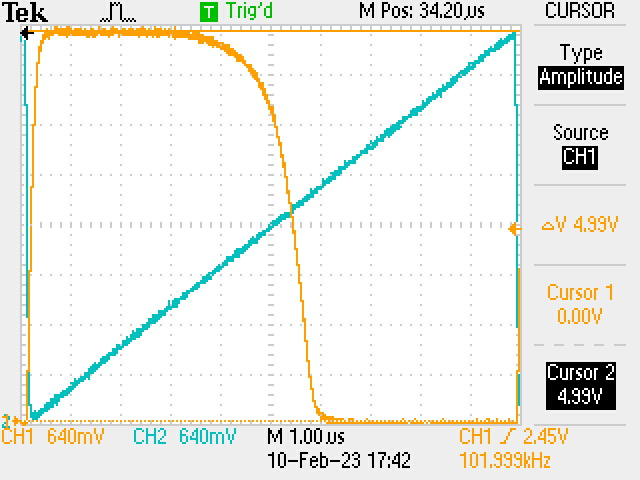
\includegraphics[scale = 0.9]{figures/rampcase1_experimental.JPG}}
    Figure 37. Ramp Case I - 5V, 100kHz, experiemtnal
\end{center} 

\subsection{Ramp Case 2 (180kHz $\leq$ f $\leq$ 200kHz)}

\begin{center}
    \centerline{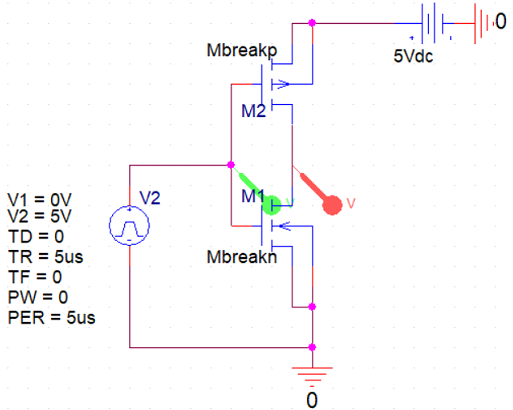
\includegraphics[scale = 0.6]{figures/rampcase2_circuit.png}}
    Figure 38. Ramp Case II - 5V Ramp input, f = 200kHz and T = 5us
\end{center}

\begin{center}
    \centerline{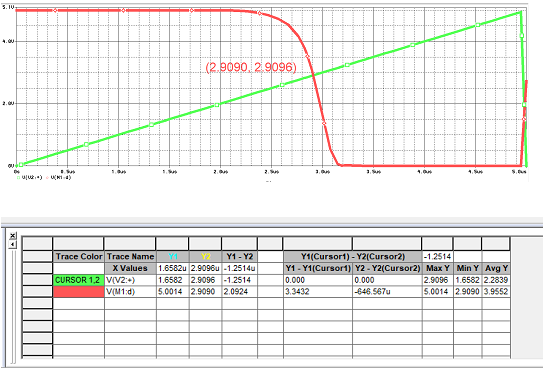
\includegraphics[scale = 0.6]{figures/rampcase2_results.png}}
    Figure 39. Ramp Case II - 5V Ramp input, f = 200kHz and T = 5us, simulation
\end{center}

\begin{center}
    \centerline{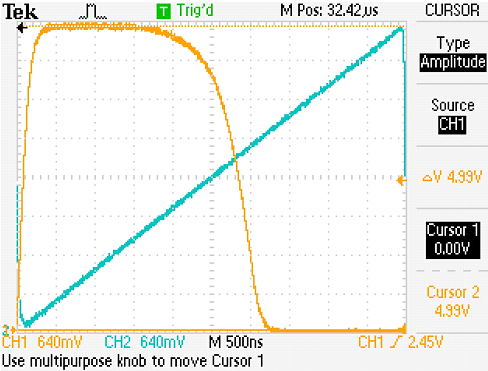
\includegraphics[scale = 0.6]{figures/rampcase2_experimental.png}}
    Figure 40. Ramp Case II - 5V Ramp input, f = 200kHz and T = 5us, experiemtnal
\end{center} 

\section{Conclusion}

\begin{thebibliography}{00}
\bibitem{b1} ECE 442L Manual
\bibitem{b2} ECE 442L supplementary slides
\bibitem{b3} Sedra, Adel S., et al. Microelectronic Circuits. Oxford University Press, 2021.
\end{thebibliography}
\vspace{12pt}
\color{red}

\end{document}